\subsection{Subchapter Title}

\bigskip

\subsubsection{Title \ldots}

\bigskip

\subsubsection{Title \ldots}

\bigskip

% Example: second diagram
\begin{diagram}[H]
  \centering
  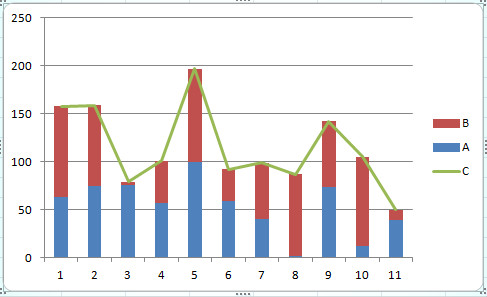
\includegraphics[width=0.7\textwidth]{images/diagram-4.2.jpg}
  \caption{Second diagram}
  \label{diag:4.2}
\end{diagram}

\subsubsection{Title \ldots}

\bigskip

% Example: second data table
\begin{table}[H]
  \centering
  \caption{Second table}
  \label{tab:4.2}
  \begin{tabular}{lccc}
    \toprule
    \textbf{Type} & \textbf{Value 1} & \textbf{Value 2} & \textbf{Value 3} \\
    \midrule
    A & 0.93 & 1.28 & 2.47 \\
    B & 0.82 & 1.39 & 2.89 \\
    C & 0.75 & 1.32 & 3.14 \\
    \bottomrule
  \end{tabular}
\end{table}
